\documentclass[12pt]{article}
\usepackage{a4wide}

\usepackage{amssymb,amsmath,amsfonts,amssymb,stmaryrd}
\usepackage{graphicx, color, url, natbib}
\usepackage{hyperref}
\usepackage{mathrsfs}
\usepackage{threeparttable}

\usepackage{graphicx, color, colortbl, texdraw, enumerate}

\newcommand{\red}[1]{\textcolor{red}{#1}}
\newcommand{\blue}[1]{\textcolor{blue}{#1}}
\newcommand{\xB}{{\bf x}}
\newcommand{\zB}{{\bf z}}
\newcommand{\YB}{{\bf Y}}
\newcommand{\AB}{{\bf A}}
\newcommand{\BB}{{\bf B}}
\newcommand{\CB}{{\bf C}}
\newcommand{\DB}{{\bf D}}
\newcommand{\IB}{{\bf I}}
\newcommand{\MB}{{\bf M}}
\newcommand{\VB}{{\bf V}}
\newcommand{\Xb}{\boldsymbol{X}}
\newcommand{\Yb}{\boldsymbol{Y}}
\newcommand{\zeroB}{{\bf 0}}
\newcommand{\thetaB}{{\boldsymbol{\theta}}}
\newcommand{\betaB}{{\boldsymbol{\beta}}}
\newcommand{\muB}{{\boldsymbol{\mu}}}
\newcommand{\SigmaB}{{\boldsymbol{\Sigma}}}
\newcommand{\DeltaB}{{\boldsymbol{\Delta}}}
\newcommand{\deltaB}{{\boldsymbol{\delta}}}
\newcommand{\E}{{\text{E}}}
\newcommand{\dint}{{\text{d}}}
\newcommand{\I}{{\text{I}}}
\newcommand{\Var}{{\text{Var}}}
\newcommand{\Cov}{{\text{Cov}}}
\newcommand{\Corr}{{\text{Corr}}}
\newcommand{\diag}{{\text{diag}}}
\newcommand{\expit}{{\text{expit}}}


\begin{document}
\title{\bf 2026 ADMTP Course on Randomization \\(Alex, Diane, Johannes, Yevgen)}

\maketitle

\thispagestyle{empty}

\vspace{-5mm}


\section*{March 5, 2026}

\begin{itemize}
    \item Alex, Diane, Johannes connected (Yevgen excused).
    \item The 2026 ADMPT workshop will take place at Newcastle University, June 1--3, 2026: \href{https://admtp.github.io/ADMTP2026/index.html}{https://admtp.github.io/ADMTP2026/index.html}
        \begin{itemize}
        \item June 1st, 9am--12:30pm: \textbf{Course 1: Practitioner’s View of Adaptive Designs}.  Course tutors: Prof. Tim Friede (Department of Medical Statistics, University of Goettingen), Dr. Hiya Banerjee(Eli Lilly) 
        \item June 1st, 2pm--5:30pm: \textbf{Course 2: Designing better trials: Advanced randomization methods for modern clinical research}.  Course tutors:  Dr. Alex Sverdlov (Novartis), Dr. Yevgen Ryeznik (Uppsala University), Dr. Diane Uschner (Roche), and Dr. Johannes Krisam (Boehringer Ingelheim), Randomisation Working Group
        \item June 2nd and 3rd, tentative agenda is as follows (Figure~\ref{Fig1}):
        \begin{figure}
            \centering
            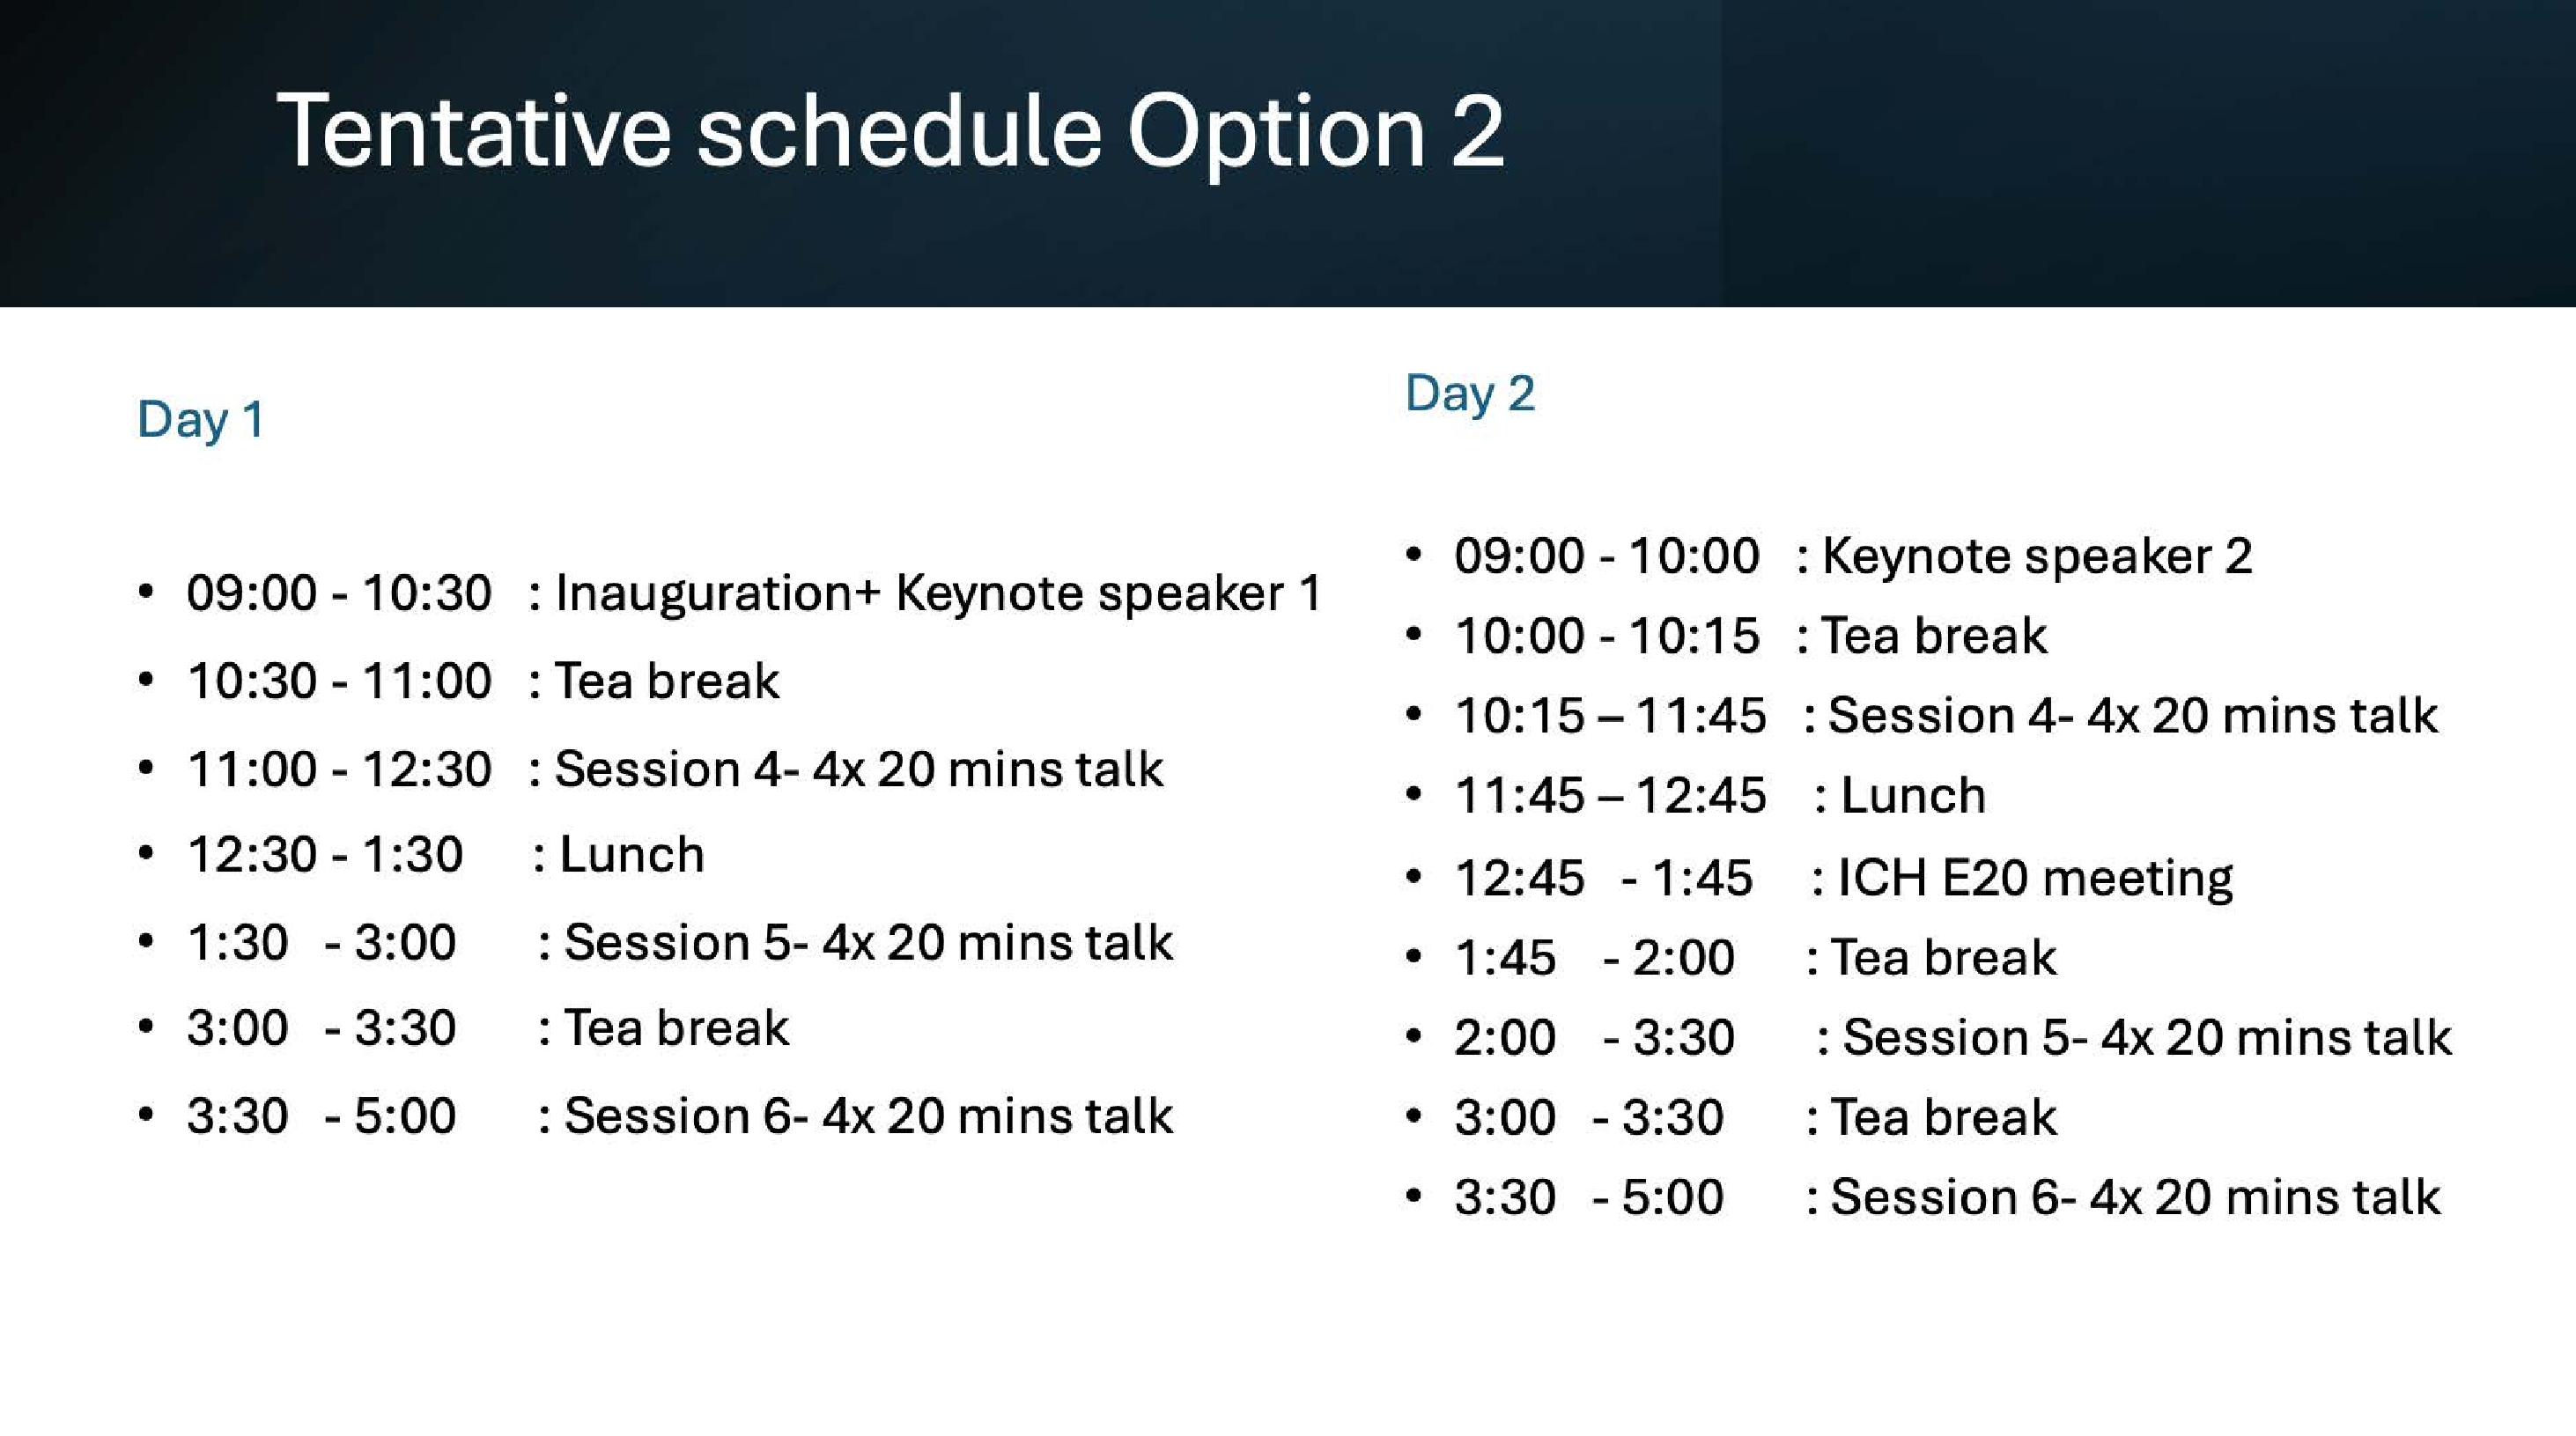
\includegraphics[width=0.5\linewidth]{=References=/ADMPT_Agenda_Day1-2.pdf}
            \caption{ADMTP Days 1--2 (tentative).}
            \label{Fig1}
        \end{figure}
    \end{itemize}
    \item We will ``divide and conquer'' the preparation of the slides/content of the short course on Randomization: 
    \begin{itemize}
        \item Diane will lead the development of \textbf{Part 1:} Introduction to Randomization: Foundations and Strategic Selection
        \item Johannes and Yevgen will co-lead the development of \textbf{Part 2:} Advanced Restricted Randomization for Multi-Arm and Platform Trials (Core Focus)
        \item Alex will lead the development of \textbf{Part 3:} Response-Adaptive Randomization (RAR): Suitability and Regulatory Landscape (Overview)
    \end{itemize}
    \item For each part, it will be important to emphasize the current regulatory considerations. Some important references to keep in mind:
    \begin{itemize}
        \item Randomization WG Comments on ICH E20 Draft Guidance Adaptive Designs for Clinical Trials: \href{https://randomization-wg.org/ich-e20-response/}{https://randomization-wg.org/ich-e20-response/}
        \item Systematic review of regulatory guidance on randomization and the use of randomization tests \citep{Carter:2024}
        \item Systematic review of RAR case studies \citep{Sverdlov:2025}
    \end{itemize}
    \item Johannes shared the materials (short course on RAR) taught by Sofía Villar and her team in 2024.
    \item We briefly discussed the 2026 FDA drat guidance, ``Use of Bayesian Methodology in Clinical Trials of Drug and Biological Products''\\
    
    \href{https://www.fda.gov/media/190505/download}{https://www.fda.gov/media/190505/download}\\
    
    It does not seem to have any mention of randomization either in the design or analysis. This may be an opportunity for us to highlight the gap. 
    \item We also discussed Bayesian Dynamic Borrowing (BDB). One important feature of BDB is that is does not provide a strong control of the Type 1 Error Rate. An important question to consider: \textbf{Does Randomization-Based Inference (RBI) make sense in the context of BDB?} How could the outcome data from historical controls (fixed, unaffected by treatment assignment in the randomization test) be handled?
    \item We acknowledged that this short course can result in various additional useful outputs, such as a Tutorial on Brick Tunnel Randomization (previously planned as a publication for \emph{Statistics in Medicine}).
    \item \textbf{Next steps:}
    \begin{enumerate}
        \item Set up bi-weekly calls to connect and check progress \textcolor{blue}{(Alex)}
        \item Decide on the state-of-the-art and fit-for-purpose technology to create the content of the course $\Rightarrow$ R Markdown, R Shiny, utilize LLMs to generate slides? \textcolor{blue}{(All)}
        \item Decide on the shared space to keep the developed content: Overleaf for Project Management, GitHub for the codes and developed content? \textcolor{blue}{(All)}
    \end{enumerate}
\end{itemize}

\begin{thebibliography}{99}

{\footnotesize

\bibitem[Carter et al., 2024]{Carter:2024} 
Carter K., Scheffold, A. L., Renteria, J., Berger, V. W., Luo, Y. A., Chipman, J. J., and Sverdlov, O. (2024). Regulatory guidance on randomization and the use of randomization tests in clinical trials: a systematic review. \emph{Statistics in Biopharmaceutical Research}, \textbf{16}(4), 428--440. \href{https://doi.org/10.1080/19466315.2023.2239521}{https://doi.org/10.1080/19466315.2023.2239521}

\bibitem[Sverdlov et al., 2025]{Sverdlov:2025} 
Sverdlov, O., Renteria, J., Carter, K., Scheffold, A. L., Krisam, J., Mascheroni, P., and Seidel, J. (2025). To what extent is response-adaptive randomization used in clinical trials? A systematic review using Cortellis Regulatory Intelligence Database. \emph{Statistical Methods in Medical Research}, \textbf{34}(9), 1875--1885.  \href{https://doi.org/10.1177/09622802251354924}{https://doi.org/10.1177/09622802251354924}

}

\end{thebibliography}

\end{document}






